\subsection{Looking Under the Hood}
Our thorough experiments over a wide range of ABR techniques indicate that DASH over QUIC does not perform as well as it is supposed to. To explore this further, we perform a set of experiments to understand the issues with QUIC, which affect DASH-based video streaming.

\subsubsection{Does QUIC Perform Poorly in All Scenarios?}
One immediate question that might arise in this context is whether the observed performance drops are generic for QUIC, or whether certain features of QUIC affect the performance of DASH. With the similar network setup as discussed before, we compute the overall throughput and the response latency for TCP and QUIC over two different scenarios -- (a) downloading of large web-objects and (b) DASH video streaming.

\newcommand{\subsubsubsection}[1]{\textbf{#1: }}
\subsubsubsection{Performance during HTTP Object Downloads}
To see how the performances of TCP and QUIC fare during the download of HTTP web objects, we perform a set of experiments over the same network setup with emulated bandwidth control via {\tt Mahimahi} traffic shaper. We download HTTP web objects (HTML and data files) of predefined sizes (from $2$MB to $50$MB) for $40$ sequential HTTP requests in each session. We give a pause of $500$ms before requesting the next web object. We repeat each session three times for both TCP and QUIC. 


\begin{figure}[!ht]
	\captionsetup[subfigure]{}
	\begin{center}
		\subfloat[\label{fig:chap03s2:proofLargeFileThroughput}Throughput]{
			\includegraphics[width=.49\linewidth]{img/proof/largefile/throughput}
		}
		\subfloat[\label{fig:chap03s2:proofLargeFileWait}Response latency]{
			\includegraphics[width=.49\linewidth]{img/proof/largefile/wait}
		}
	\end{center}
	\caption{\label{fig:chap03s2:proofLargeFile}TCP and QUIC performance during HTTP web object download}
\end{figure}


Fig.~\ref{fig:chap03s2:proofLargeFileThroughput} shows the distribution of throughput observed against each web object downloads, while Fig.~\ref{fig:chap03s2:proofLargeFileWait} indicates the response latency observed by each HTTP request. The throughput is computed as the object size divided by the download time where the download time is the time difference between the first and the last bytes received for that web object. The response latency is computed as the time between the initiation of the HTTP request and the time when the first byte of the response is received. From the figures, we see that the throughput is similar for HTTP/TCP and HTTP/QUIC. The response latency for HTTP/QUIC is slightly lower than HTTP/TCP. These experiments shows that QUIC performs better than TCP in terms of response latency which is an important QoE metric for web object downloads. 


\begin{figure}[!ht]
	\captionsetup[subfigure]{}
	\begin{center}
		\subfloat[\label{fig:chap03s2:proofCompThroughput} Throughput ]{
			\includegraphics[width=.45\linewidth]{img/proof/comp/throughput}
		}
		\hfill
		\subfloat[\label{fig:chap03s2:proofCompWait} Response latency]{
			\includegraphics[width=.45\linewidth]{img/proof/comp/wait}
		}
	\end{center}
	\caption{\label{fig:chap03s2:dashcomp}TCP and QUIC performance during DASH video segment download}
\end{figure}


\subsubsubsection{Performance during Video Streaming}
Fig.~\ref{fig:chap03s2:proofCompThroughput} shows the distribution of the throughput observed during the video playback, combining the data from all the five ABR mechanisms. A statistical test also indicates that the difference between TCP and QUIC in terms of throughput is not significant. Interestingly, the predicted throughput during video streaming is one of the important metrics used by all the ABR mechanisms for deciding the optimal bitrate. Fig.~\ref{fig:chap03s2:proofCompWait} plots the distributions of the response latency, combining the videos from all the five ABR mechanisms. We have an interesting observation here -- although the difference in the median of the response latency for DASH/QUIC and DASH/TCP is not significant,  the upper quartile for the response latency of DASH/QUIC is significantly higher than the upper quartile of DASH/TCP. This indicates that with QUIC, the response latency sometime becomes very high -- this observation is opposite to what we have observed in Fig.~\ref{fig:chap03s2:proofLargeFileWait}. It can be noted that the throughput computation does not consider the response latency, rather it considers the time difference between the first and the last bytes received for a video segment. The ABR algorithms primarily select the bitrate based on the computed throughput for the last few video segments. If the computed throughput is high, the DASH client requests for the next video segment in an increased quality level. However, if the response latency is high, this segment may take longer time to reach the client, resulting in a rebuffering and subsequent drop in the quality levels for the next video segments. We do not see this problem for TCP, as the response latency correlates with the computed throughput; however, this correlation does not hold for QUIC. Next, we dig further to find out the reason behind the high response latency observed during the video streaming using QUIC.

\subsubsection{Exploring TCP and QUIC Connections during a Video Streaming}
During the dashification of a video with an embedded audio, the standard practice is to first segregate and segment the video data and the corresponding audio data, and then encode the video and the audio segments separately in their respective available encoding formats.
Now the DASH client creates two different HTTP streams for downloading the video segments and the corresponding audio segments. For DASH/TCP, two different TCP sockets are created between the DASH client and the server for these two HTTP streams, whereas for DASH/QUIC, both the HTTP streams are multiplexed, and the HTTP messages are exchanged over a single UDP socket.
This brings the next question -- how do TCP and QUIC fare for two parallel but interdependent application streams between the same client and the server?  To answer this question, we do the next experiment over the same network setup as discussed before. In this experiment, we create two HTTP streams where both the streams request for the HTTP objects (files) in parallel. The object sizes are varied from $1$MB to $8$MB.
We also vary the duration between two HTTP requests (called the pause time) from $500$ms to $8000$ms. 

\begin{figure}[!ht]
	\captionsetup[subfigure]{}
	\begin{center}
		\subfloat[\label{fig:chap03s2:proofUhoodMThroughput2} Throughput]{
			\includegraphics[width=.49\linewidth]{img/proof/uhoodM/throughput-2}
		}
		\subfloat[\label{fig:chap03s2:proofUhoodMWait2} Response latency ($p<0.05$ for all the instances)]{
			\includegraphics[width=.49\linewidth]{img/proof/uhoodM/wait-2}
		}
	\end{center}
	\caption{\label{fig:chap03s2:proofUhoodM}Performance of TCP and QUIC for two parallel connections}
\end{figure}


Fig.~\ref{fig:chap03s2:proofUhoodM} shows the observations from this experiment. The differences in throughput between QUIC and TCP is not significant; however, the response latency with QUIC is significantly higher than TCP when two parallel application streams generate HTTP requests. Further, this difference in the response latency is more prominent when the pause time is less indicating the frequency of the HTTP requests is high. This observation is very synonymous to what we observed in Fig.~\ref{fig:chap03s2:dashcomp}. To find out the reason for such a behavior, we see that the problem is inherited from the behavior of the socket buffers used to interface between the user-space and the kernel-space. As TCP creates two separate sockets for the two HTTP streams, each of the sockets maintains its own socket buffer. Therefore, the HTTP responses from the two streams do not interfere with each other. On the other hand, QUIC multiplexes both the streams and uses a single UDP socket having a single socket buffer. Therefore, the HTTP responses from both the streams interfere, and higher response rate at one stream affects the queuing delay for the response at the other stream. 


When DASH uses two separate HTTP streams for video and audio downloads, the stream corresponding to the video downloads has a higher data generation rate compared to the stream corresponding to the audio download. This is because the amount of video data to be downloaded is much higher compared to the amount of the audio data to be downloaded, for a fixed playback time. For DASH/TCP, the audio and the video streams use separate socket buffers, having independent queuing delay depending on their data generation rate. However, for QUIC, both the streams get multiplexed. For every playback segment, the client generates one HTTP request for the video segment and another HTTP request for the audio segment. As the video segment request is sent first, the UDP socket buffer gets filled up with the majority of the video segment data. Consequently, the data for the audio segment needs to wait until that video data gets freed up from the socket buffer. Fig.~\ref{fig:chap03s2:proofCompDlTime} shows an example instance of video download using QUIC, where we see that video data is served almost immediately after the request is received at the server. However, the audio data has to wait in the queue (the red timeline) before it gets served. This problem is not there in TCP as the fairness property of TCP flow and congestion control serves both the socket buffers in a fair way. So, the audio data does not experience this high response latency. Fig.~\ref{fig:chap03s2:proofCompAVLatency} shows the distributions of the response latency for the audio and video streams separately. We see that the distributions of the response latency for the video streams are similar for QUIC and TCP. However, the audio streams at QUIC experiences a much higher latency compared to TCP. 


\begin{figure}[!ht]
	\captionsetup[subfigure]{}
	\begin{center}
   		\subfloat[\label{fig:chap03s2:proofCompDlTime} Video/Audio downloads over QUIC]{
   			\includegraphics[width=.45\linewidth]{img/proof/comp/ls}
   		}
           		\hfill
		\subfloat[\label{fig:chap03s2:proofCompAVLatency} Response latency for audio and video]{
			\includegraphics[width=.45\linewidth]{img/proof/comp/avwait}
		}
	\end{center}
	\label{fig:chap03s2:dashcompres}
	\caption{TCP and QUIC response latency during video and audio downloads over separate streams}
\end{figure}


\subsection{Summary}
We observe that during parallel downloads of audio and video streams, QUIC multiplexing affects the response latency of the audio streams. This observation also tallies with the observation made in~\cite{kakhki2019taking}, which states that multiplexing objects from parallel streams affect the latency of individual objects. This latency is inevitable because of multiplexing multiple objects over a single UDP queue, whereas the final video playback depends on the successful download of both the video and the audio segments. Interestingly, the throughput calculation used in DASH does not consider this response latency, resulting in a mismatch between the expected throughput and the actual download time of the segments after a request is sent. There might not be a direct solution to this problem as DASH is unaware of such behaviors of the underlying data transmission protocol, whereas QUIC is unaware of the dependency between the audio and the video streams for successful streaming of the video. We might need further investigation of the QUIC protocol stack to make it compatible with the state-of-the-art ABR streaming mechanisms.  

Apart from the protocol choices, mobility plays another important role during video streaming over smartphones. Till now, we considered the network bandwidth as the only factor for video streaming; however, as video streaming is a network-intensive application, and peoples across the globe use video streaming applications widely over smartphones, energy consumption becomes another concern. Therefore, in the next section, we investigate how video streaming applications impact the device's energy consumption due to their network-intensive activities.  




